\chapter{Airborne collision avoidance system} \label{chap:acas}

\section{Background}

\emph{Airborne Collision Avoidance System} (ACAS) is a system to reduce the risk of mid-air collisions and near mid-air collisions between aircraft. There are three types of ACAS systems according to \cite{icaoA10V4}, which are:

\begin{itemize}
  \item ACAS I: Gives traffic advisories (TA), without recommending manoeuvres.
  \item ACAS II: Gives traffic advisories (TA) and resolution advisories (RA) only in vertical directions.
  \item ACAS III: Gives traffic advisories (TA) and resolution advisories (RA) in both horizontal and vertical directions. ACAS III is not currently implemented
\end{itemize}

This chapter will focus on ACAS II. The ACAS II is a system that utilizes the aircraft transponder, which interrogates the Mode~C and Mode~S transponders of nearby aircraft. When threats are detected, corresponding alerts are given to the pilots.

Currently, the most common implementation of ACAS II is \emph{Traffic alert and Collision Avoidance System} (TCAS) II version 7.1, which was initiated by EUROCONTROL. It has been mandatory for aircraft in Europe since 2015. ACAS II works independently of the navigation system, FMS, and ATC. No input from these systems is considered for producing the alerts. 


\begin{notebox}{Note}
In the future, a new system developed by FAA, called `ACAS X', is expected to replace the current ACAS II. It makes use of dynamic programming to generate resolution advisories and offers four performance capability variants for different air traffic scenarios. \cite{chomik2016}
\end{notebox}
  

In ACAS II, TA and RA are triggered when certain thresholds to the closest point of approach (CPA) are passed. The thresholds depend on the altitude, speed, and heading of the aircraft. The examples of the TA and RA regions are illustrated in Figure \ref{fig:acas_regions}.

\begin{figure}[ht]
\centering
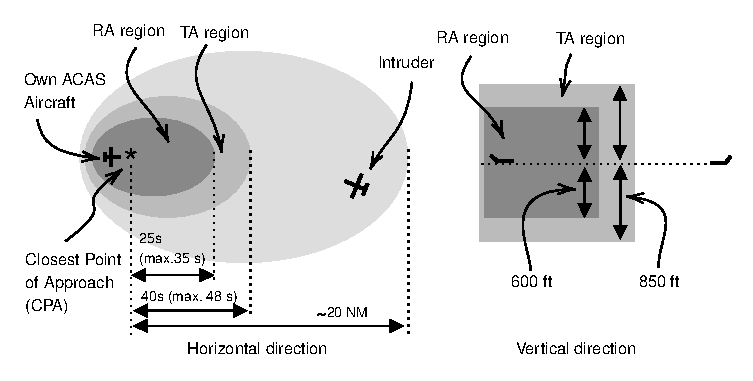
\includegraphics[scale=0.9]{figures/mode_s/acas_regions.pdf}
\caption{Example of an ACAS protection volume in horizontal and vertical directions (between FL50 and FL100)}
\label{fig:acas_regions}
\end{figure}




\section{ACAS with Mode~C transponders}

The ACAS system uses Mode~C only all-call interrogation to detect aircraft that are only equipped with Mode~A/C transponders. In this case, the ACAS system initiates a sequence of interrogations with increasing power.

The interrogation pulse is slightly different from a Mode~A/C-only all-call interrogation. A special $S_1$ pulse (also known as `whisper-shout') is designed to reduce interference. The $S_1$ pulse is inserted 2  μs ($\pm 0.15 \mu s$) before the $P_1$ pulse.

The reply should be sent with the following rules:

\begin{itemize}
  \item With both $S_1$ and $P_1$ above the minimum triggering level (MTL), no reply will be generated.
  \item With both $S_1$ and $P_1$ at MTL, the transponder will respond to 10\% of the interrogations.
  \item With $P_1$ at MTL and $S_1$ at MTL - 3 dB, the transponder will respond to 70\% of the interrogations.
  \item With $P_1$ at MTL and $S_1$ at MTL - 6 dB, the transponder will respond to 90\% of the interrogations.
\end{itemize}

\section{ACAS with Mode~S transponders}

For Mode~S transponders, the ACAS system employs a three-phase process, which includes the phases of \emph{detection}, \emph{surveillance}, and \emph{coordination}.

For the detection phase, ACAS passively listens to Mode~S only all-call replies (DF=11). These all-call replies are usually generated as a result of ground SSR interrogations, or created by spontaneous acquisition squitter (broadcast of DF=11 message with interrogator code \texttt{0}). In this process, aircraft with Mode~S transponders in the vicinity are discovered. ACAS may also listen to extended squitter messages (Downlink Format 17, ADS-B) to detect other aircraft.

Once another aircraft is determined to be within the ACAS surveillance range, and within 10,000 ft of the own aircraft\footnote{This can be acquired through existing DF=0 and DF=4 replies, or through active interrogations}, ACAS will initiate a short air-air interrogation (UF=0) to acquire the range. The interrogation rate is defined as:

\begin{itemize}
  \item Once every five cycles: when the target aircraft remains in the surveillance range.
  \item Once every cycle: when the target aircraft is within 3 NM or with time to closest approach less than 60 s.
\end{itemize}


The surveillance interrogation is stopped when all the following conditions are met:

\begin{itemize}
  \item A reply (DF=0) is received
  \item Both aircraft are below 18,000 ft.
  \item Target aircraft is more than 3 NM and 60 s away from the closest point of approach.
\end{itemize}


Tables \ref{tb:acas_uf_0} and \ref{tb:acas_df_0} lists the fields for ACAS surveillance interrogation and reply messages.

\begin{table}[ht]
  \centering
  \caption{ACAS surveillance interrogation (uplink), UF=0}
  \label{tb:acas_uf_0}
  \begin{tabular}[t]{|l|l|l|l|}
  \hline
  \textbf{FIELD} & \textbf{} & \textbf{MSG} & \textbf{BITS} \\ \hline
  Uplink Format & UF & 1--5 & 5 \\ \hline
  Reserved &  & 6--8 & 3 \\ \hline
  Reply length & RL & 9 & 1 \\ \hline
  Reserved &  & 10--13 & 4 \\ \hline
  Acquisition & AQ & 14 & 1 \\ \hline
  Data selector & DS & 15--22 & 8 \\ \hline
  Reserved &  & 23--32 & 10 \\ \hline
  Address parity & AP & 33--56 & 24 \\ \hline
  \end{tabular}
\end{table}


\begin{table}[ht]
  \centering
  \caption{ACAS surveillance reply (downlink), DF=0}
  \label{tb:acas_df_0}
  \begin{tabular}[t]{|l|l|l|l|}
  \hline
  \textbf{FIELD} & \textbf{} & \textbf{MSG} & \textbf{BITS} \\ \hline
  Downlink Format & DF & 1--5 & 5 \\ \hline
  Vertical status & VS & 6 & 1 \\ \hline
  Cross-link capability & CC & 7 & 1 \\ \hline
  Reserved &  & 8 & 1 \\ \hline
  Sensitivity level & SL & 9--11 & 3 \\ \hline
  Reserved &  & 12--13 & 2 \\ \hline
  Reply information & RI & 14--17 & 4 \\ \hline
  Reserved &  & 18--19 & 2 \\ \hline
  Altitude code & AC & 20--32 & 13 \\ \hline
  Address parity & AP & 33--56 & 24 \\ \hline
  \end{tabular}
\end{table}


Once the target aircraft is within the RA region (a threat), ACAS initiates the coordination interrogation (UF=16). In this step, resolution information are transmitted and received through coordination replies (DF=16). Information that is included in both coordination messages is shown in Tables \ref{tb:acas_uf_16} and \ref{tb:acas_df_16}.


\begin{table}[ht]
  \centering
  \caption{ACAS coordination interrogation (UF=16)}
  \label{tb:acas_uf_16}
  \begin{tabular}[t]{|l|l|l|l|}
  \hline
  \textbf{FIELD} & \textbf{} & \textbf{MSG} & \textbf{BITS} \\ \hline
  Uplink Format & UF & 1--5 & 5 \\ \hline
  Reserved &  & 6--8 & 3 \\ \hline
  Reply length & RL & 9 & 1 \\ \hline
  Reserved &  & 10--13 & 4 \\ \hline
  Acquisition & AQ & 14 & 1 \\ \hline
  Reserved &  & 15--32 & 18 \\ \hline
  Message, U & MU & 33--88 & 56 \\ \hline
  Address parity & AP & 33--56 & 24 \\ \hline
  \end{tabular}
\end{table}%

\begin{table}[ht]
  \centering
  \caption{ACAS coordination reply (DF=16)}
  \label{tb:acas_df_16}
  \begin{tabular}[t]{|l|l|l|l|}
  \hline
  \textbf{FIELD} & \textbf{} & \textbf{MSG} & \textbf{BITS} \\ \hline
  Downlink Format & DF & 1--5 & 5 \\ \hline
  Vertical status & VS & 6 & 1 \\ \hline
  Reserved &  & 7--8 & 2 \\ \hline
  Sensitivity level & SL & 9--11 & 3 \\ \hline
  Reserved &  & 12--13 & 2 \\ \hline
  Reply information & RI & 14--17 & 4 \\ \hline
  Reserved &  & 18--19 & 2 \\ \hline
  Altitude code & AC & 20--32 & 13 \\ \hline
  Message, V & MV & 33--88 & 56 \\ \hline
  Address parity & AP & 89--112 & 24 \\ \hline
  \end{tabular}
\end{table}


Specific fields in the above mentioned messages are defined as follows:

\begin{itemize}
  \item \emph{Reply length (RL)}: 1 bit, it defines the required reply format: \texttt{0} requires a reply with DF=0, while \texttt{1} requires reply with DF=16.

  \item \emph{Acquisition (AQ)}: 1 bit, it contains code that controls the content of RI field in the reply.

  \item \emph{Data selector (DS)}: 8 bits, it indicates the BDS code of the MV content in reply with DF=16.

  \item \emph{Vertical status (VS)}: 1 bit, it indicates whether the aircraft is airborne (\texttt{0}) or on the ground (\texttt{1}).

  \item \emph{Cross-link capability (CC)}: 1 bit, it refers to the capability of reply DF=16 upon request of UF=0. When this 1-bit field is set to \texttt{1}, the cross-link is supported. Otherwise, the field is set to \texttt{0}.

  \item \emph{Sensitivity level (SL)}: 3 bits, it represents the sensitivity level of the ACAS system, except that \texttt{0} indicates the ACAS is inoperative.

  \item \emph{Reply information (RI)}: 4 bits, it indicates the type of reply to interrogating aircraft. For ACAS message, valid values are 0 and from 2 to 4. Other values are not part of the ACAS:

  \begin{quote}
    \texttt{0000}: No operating ACAS \\
    \texttt{0010}: ACAS with resolution capability inhibited \\
    \texttt{0011}: ACAS with vertical-only resolution capability \\
    \texttt{0111}: ACAS with vertical and horizontal resolution capability
  \end{quote}

  \item \emph{Altitude Code (AC)}: 13 bits, it encodes the altitude of the aircraft. It can be decoded according to section \ref{sec:alt_code}.

\end{itemize}



\section{ACAS coordination interrogation}

Message U-definition (MU) is transmitted in ACAS coordination interrogation. MU is used to transit resolution, ACAS broadcast, and RA broadcast.


\subsection{UDS=3,0}

When ACAS resolution information is transmitted in the UF=16 message, the first 8 bits of MU, U-definition subfields (UDS), are set to \texttt{0011 0000} (UDS=3,0). The corresponding fields are indicated in Table \ref{tb:acas_mu_uds30}.

\begin{table}[ht]
\caption{UF=16, MU for ACAS resolution messages, UDS=3,0}
\label{tb:acas_mu_uds30}
\begin{tabular}{|l|l|l|l|l|}
\hline
\textbf{FIELD} & \textbf{} & \textbf{MSG} & \textbf{MU} & \textbf{BITS} \\ \hline
U-definition subfield 1 [0011] & UDS1 & 33--36 & 1--4 & 4 \\ \hline
U-definition subfield 2 [0000] & UDS2 & 37--40 & 5--8 & 4 \\ \hline
Reserved &  & 41 & 9 & 1 \\ \hline
Multiple threat bit & MTB & 42 & 10 & 1 \\ \hline
Cancel vertical RAC & CVC & 43--44 & 11--12 & 2 \\ \hline
Vertical RAC & VRC & 45--46 & 13--14 & 2 \\ \hline
Cancel Horizontal RAC & CHC & 47--49 & 15--17 & 3 \\ \hline
Horizontal RAC & HRC & 50--52 & 18--20 & 3 \\ \hline
Reserved &  & 53--55 & 21--23 & 3 \\ \hline
Horizontal sense bits & HSB & 56--60 & 24--28 & 5 \\ \hline
Vertical sense bits & VSB & 61--64 & 29--32 & 4 \\ \hline
Aircraft address & MID & 65--88 & 33--56 & 24 \\ \hline
\end{tabular}
\end{table}

These fields can be interpreted as follows:

\begin{itemize}
  \item \emph{Multiple threat bit (MTB)}: 1 bit, indicates whether multiple threats are present.

  \item \emph{Vertical RAC \footnote{RAC: Resolution Advisory Complement} (VRC)}: 2 bits, contains vertical resolution advisory complement information:
  \begin{quote}
    \small
    \texttt{00}: No vertical RAC information \\
    \texttt{01}: Do not pass below \\
    \texttt{10}: Do not pass above \\
    \texttt{11}: Not assigned
  \end{quote}

  \item \emph{Cancel vertical RAC (CVC)}: 2 bits, cancels previously sent VRC:
  \begin{quote}
    \small
    \texttt{00}: No cancellation information \\
    \texttt{01}: Cancel "Do not pass below" \\
    \texttt{10}: Cancel "Do not pass above" \\
    \texttt{11}: Not assigned
  \end{quote}

  \item \emph{Horizontal RAC (HRC)}: 3 bits, contains horizontal resolution advisory complementary information:
  \begin{quote}
    \small
    \texttt{000}: No information\\
    \texttt{001}: Other ACAS sense is turn left; do not turn left \\
    \texttt{010}: Other ACAS sense is turn left; do not turn right \\
    \texttt{101}: Other ACAS sense is turn right; do not turn left \\
    \texttt{110}: Other ACAS sense is turn right; do not turn right \\
    \texttt{other}: Not assigned
  \end{quote}

  \item \emph{Cancel horizontal RAC (CHC)}: 3 bits, cancels previously sent HRC:
  \begin{quote}
    \small
    \texttt{000}: No cancellation information \\
    \texttt{001}: Cancel "Do not turn left" \\
    \texttt{010}: Cancel "Do not turn right" \\
    \texttt{other}: Not assigned
  \end{quote}

  \item \emph{Horizontal sense bits (HSB)}: 5 bits, uses Hamming code with an extra parity bit to detect errors (up to 3 bits) in CHC and HRC fields.

  \item \emph{Vertical sense bits (VSB)}: 4 bits, uses Hamming code with an extra parity bit to detect errors (up to 3 bits) in CVC and VRC fields.

  \item \emph{Aircraft address (MID)}: 24 bits, contains the 24-bits aircraft transponder address of the interrogating ACAS aircraft.

\end{itemize}



\subsection{UDS=3,1} \label{sec:acas_ra}

When UF=16 is used for RA broadcast, UDS is set to \texttt{0011 0001} (UDS=3,1). The corresponding fields are described in Table \ref{tb:acas_mu_uds31}.

\begin{table}[ht]
\caption{UF=16, MU for RA broadcast, UDS=3,1}
\label{tb:acas_mu_uds31}
\begin{tabular}{|l|l|l|l|l|}
\hline
\textbf{FIELD} & \textbf{} & \textbf{MSG} & \textbf{MU} & \textbf{BITS} \\ \hline
U-definition subfield 1 [0011] & UDS1 & 33--36 & 1--4 & 4 \\ \hline
U-definition subfield 2 [0001] & UDS2 & 37--40 & 5--8 & 4 \\ \hline
Active RAs & ARA & 41--54 & 9--22 & 14 \\ \hline
RAC's record & RAC & 55--58 & 23--26 & 4 \\ \hline
RA terminated indicator & RAT & 59 & 27 & 1 \\ \hline
Multiple threat encounter & MTE & 60 & 28 & 1 \\ \hline
Reserved &  & 61--62 & 29--30 & 2 \\ \hline
Mode~A identity code & AID & 63--75 & 31--43 & 13 \\ \hline
Mode~C altitude code & CAC & 76--88 & 44--56 & 13 \\ \hline
\end{tabular}
\end{table}

These fields can be interpreted as follows:

\begin{itemize}
  \item \emph{Active RA (ARA)}: 14 bits, indicates the resolution advisory characteristics. It has to be interpreted together with the MTB field.

    \begin{itemize}
      \item When ARA first bit (MSG bit 41) is \texttt{1} and MTE is either \texttt{0} or \texttt{1}:

      \begin{quote}
        \small
        Bit 42: RA is corrective (\texttt{1}) or preventive (\texttt{0}) \\
        Bit 43: RA is downward sense (\texttt{1}) or upward sense (\texttt{0}) \\
        Bit 44: RA is increased rate (\texttt{1}) or not (\texttt{0}) \\
        Bit 45: RA is a sense reversal (\texttt{1}) or not (\texttt{0}) \\
        Bit 46: RA is altitude crossing (\texttt{1}) or not (\texttt{0}) \\
        Bit 47: RA is positive (\texttt{1}) or vertical speed limit (\texttt{0}) \\
        Bit 48--54: Reserved for ACAS III
      \end{quote}

      \item When ARA first bit (MSG bit 41) is \texttt{0} and MTE is \texttt{1}:

      \begin{quote}
        \small
        Bit 42: RA requires a correction in the upward sense (\texttt{1}) or not (\texttt{0}) \\
        Bit 43: RA requires a positive climb (\texttt{1}) or not (\texttt{0}) \\
        Bit 44: RA requires a correction in the downward sense (\texttt{1}) or not (\texttt{0}) \\
        Bit 45: RA requires a positive descent (\texttt{1}) or not (\texttt{0}) \\
        Bit 46: RA requires a crossing (\texttt{1}) or not (\texttt{0}) \\
        Bit 47: RA is a sense reversal (\texttt{1}) or not (\texttt{0}) \\
        Bit 48--54: Reserved for ACAS III
      \end{quote}

      \item When ARA first bit (MSG bit 41) is \texttt{0} and MTE is \texttt{0}, no vertical RA is generated.
    \end{itemize}


  \item \emph{RAC's record (RAC)}: 4 bits, contains current active RACs that are received from other ACAS aircraft (if any). Each of the four bits in this field indicates the following RAC when set to \texttt{1}. When a bit is set to \texttt{0}, the corresponding RAC is inactive.

  \begin{quote}
    \small
    Bit 55: Do not pass below \\
    Bit 56: Do not pass above \\
    Bit 57: Do not pass left \\
    Bit 58: Do not pass right
  \end{quote}


  \item \emph{RA terminated indicator (RAT)}: 1 bit, indicates whether ACAS is currently generating RA in the ARA field or RA in the ARA field has been terminated.\footnote{The Mode~S transponder is still required to report RA 18 seconds after it is terminated by ACAS. Hence, the RAT field is used.}


  \item \emph{Multiple threat encounter (MTE)}: 1 bit, indicates whether multiple threats are currently being processed by the ACAS resolution. When MTE is set to \texttt{0}, either one threat is being processed (ARA bit 41 sets to \texttt{1}) or no threat is being processed (ARA bit 41 sets to \texttt{0}). When MTE is set to \texttt{1}, multiple threats are being processed.

  \item \emph{Mode~A identity code (AID)}: 13 bits, contains the Mode~A identity code (sqwake code) of the reporting aircraft. It can be decoded according to section \ref{sec:id_code}.

  \item \emph{Mode~C altitude code (CAC)}: 13 bits, contains the Mode~C altitude code reporting aircraft. It can be decoded according to section \ref{sec:alt_code}.


\end{itemize}



\subsection{UDS=3,2}

When UF=16 is used for ACAS broadcast, UDS is set to \texttt{0011 0010} (UDS=3,2). The corresponding fields are indicated in Table \ref{tb:acas_mu_uds32}.

\begin{table}[ht]
\caption{UF=16, MU for ACAS broadcast, UDS=3,1}
\label{tb:acas_mu_uds32}
\begin{tabular}{|l|l|l|l|l|}
\hline
\textbf{FIELD} & \textbf{} & \textbf{MSG} & \textbf{MU} & \textbf{BITS} \\ \hline
U-definition subfield 1 [0011] & UDS1 & 33--36 & 1--4 & 4 \\ \hline
U-definition subfield 2 [0010] & UDS2 & 37--40 & 5--8 & 4 \\ \hline
Reserved &  & 41--64 & 9--32 & 24 \\ \hline
Aircraft address & MID & 65--8 & 33--56 & 24 \\ \hline
\end{tabular}
\end{table}

The only information that is broadcast in the MU of this message is the 24-bit transponder address of the interrogating aircraft. Its purpose is to inform other aircraft about ACAS capability of the broadcasting aircraft.


\section{ACAS coordination reply}

Message V-definition (MV) is transmitted in ACAS coordination reply message. 

\subsection{VDS=3,0}
Similar to MU in the UF=16 message, MV in the DF=16 message contains a few common fields. The corresponding fields are indicated in Table \ref{tb:acas_mv_vds30}.

\begin{table}[ht]
\caption{DF=16, MV for coordinated reply, VDS=3,0}
\label{tb:acas_mv_vds30}
\begin{tabular}{|l|l|l|l|l|}
\hline
\textbf{FIELD} & \textbf{} & \textbf{MSG} & \textbf{MV} & \textbf{BITS} \\ \hline
V-definition subfield 1 [0011] & VDS1 & 33--36 & 1--4 & 4 \\ \hline
V-definition subfield 2 [0000] & VDS2 & 37--40 & 5--8 & 4 \\ \hline
Active RAs & ARA & 41--54 & 9--22 & 14 \\ \hline
RAC's record & RAC & 55--58 & 23--26 & 4 \\ \hline
RA terminated indicator & RAT & 59 & 27 & 1 \\ \hline
Multiple threat encounter & MTE & 60 & 28 & 1 \\ \hline
Reserved &  & 61--88 & 29--56 & 28 \\ \hline
\end{tabular}
\end{table}

We can see that the structure of the MV fields is similar to MU fields of RA broadcast (UDS=3,1) from Table \ref{tb:acas_mu_uds31}. The interpretations of these fields are also the same as in section \ref{sec:acas_ra}.

\subsection{Other VDS}
When the first eight bits are not \texttt{0011 0000}, the MV field contain the Ground-initiated Comm-B information that was requested in DS field of uplink (UF=0) in Table \ref{tb:acas_uf_0}. Comm-B will be explained in the next chapter.

% It is worth noting that the DS value is not transmitted in the MV field. Thus, it is difficult to know what data is contained in the MV field for VDS other than \texttt{3,0}.
